%----------------------------------------
% Preamble to set up the document
%----------------------------------------
\documentclass{article}

% set up packages (you shouldn't need to touch this)
\usepackage{graphicx}  % required to insert images
\usepackage{hyperref}  % for hyperlinks
\usepackage[svgnames]{xcolor}  % to change hyperlink colors
\colorlet{linkcolour}{DarkBlue}
\hypersetup{colorlinks=true, linkcolor=linkcolour, citecolor=linkcolour, urlcolor=linkcolour,}

% Margins
\topmargin=-0.45in
\evensidemargin=0in
\oddsidemargin=0in
\textwidth=6.5in
\textheight=9.0in
\headsep=0.25in

% use a sans serif font
\renewcommand{\familydefault}{\sfdefault}

%----------------------------------------
% Step 1: Edit the lecture title
%----------------------------------------
\title{
Lecture 11: Networks II (Counting on Graphs), Causality and Experiments \\  % Lecture title
Modeling Social Data, Spring 2019 \\   % Course title
Columbia University                    % School
}

%----------------------------------------
% Step 2: Edit your name and the date
%----------------------------------------
\author{Deniz Ulcay}                     % Scribe's name
\date{April 12, 2019}                % Lecture date

\begin{document}

\maketitle


%----------------------------------------
% Step 3:
% Rename uni.tex to match your uni,
% edit the filename accordingly below,
% and put your notes in this file
%----------------------------------------
%----------------------------------------
% Write your notes here
%----------------------------------------

\section{Introduction}
In this lecture, we covered the following key topics:
\begin{itemize}
  \item Network Representations (Data Structures)
  \item Network Topologies and Watts-Strogatz Networks
  \item Describing Networks
  \item Causality and (Natural) Experiments
\end{itemize}

\section{Network Representations (Data Structures)}
We discussed three different data structures that can be used to represent networks: Edge list, adjacency matrix and adjacency list.

\subsection{Edge List}
One way to represent a network is a list of $|E|$ edges, called an edge list. Each edge is represented as a tuple of the two vertices the edge is incident on. Even though edge lists are simple to store, performing computations on them can be difficult. The space complexity of an edge list is $\Theta(E)$. If we wanted to check whether an edge exists between two vertices, we would need to search the entire list, which would take $O(E)$ time.

\begin{figure}[ht]
  \begin{center}
    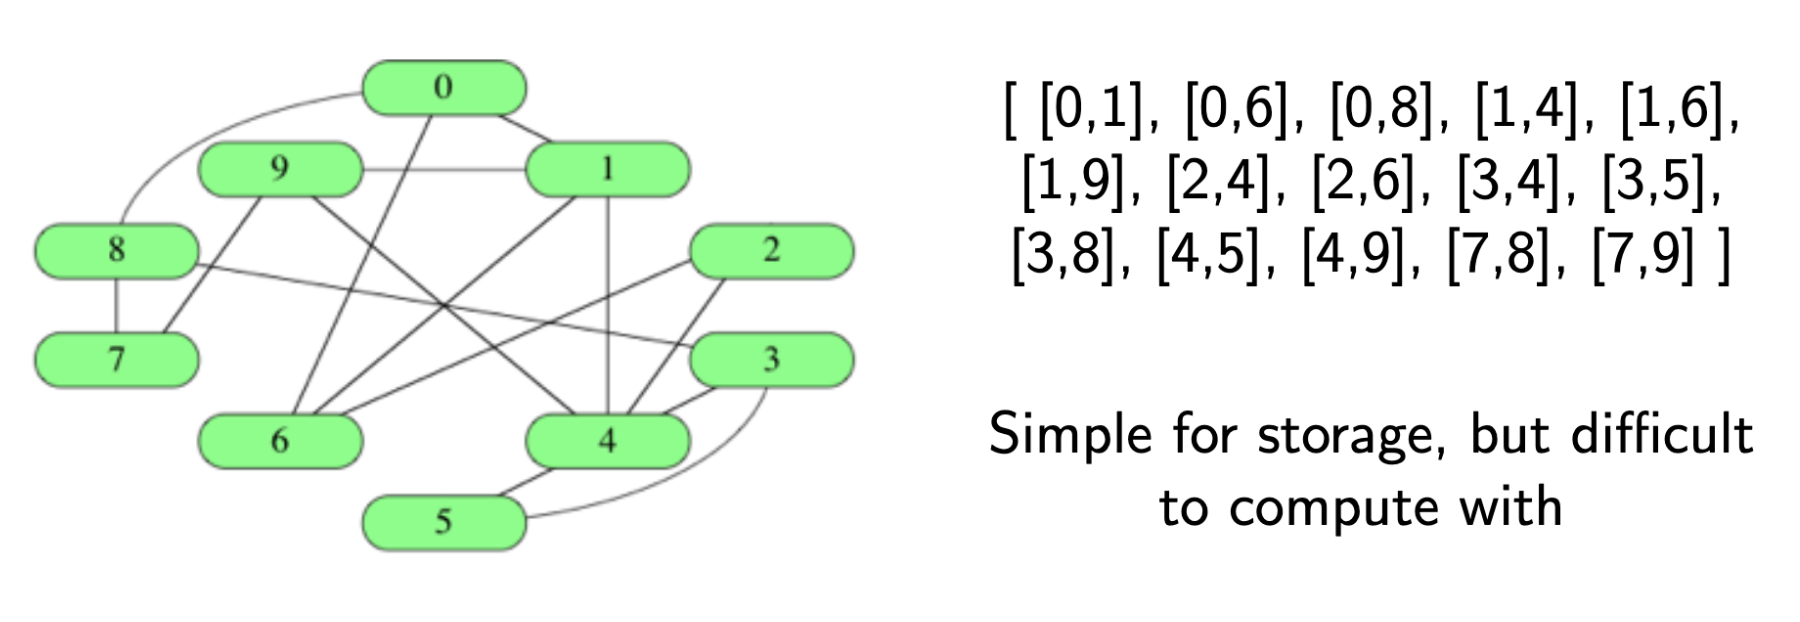
\includegraphics[width=0.5\textwidth]{figures/edge_list.png}
    \caption{
      A network with 10 vertices (left) and the edge list representation of its edges (right).}
    \label{fig:edge_list}
  \end{center}
\end{figure}

\subsection{Adjacency Matrix}
The second approach involves building a $|V|x|V|$ matrix of 1s and 0s for a network with $|V|$ vertices where row i, column j is 1 if there exists an edge between vertices i and j. The space complexity of an adjacency matrix is $\Theta(V^{2})$. Thus, if our network was relatively sparse, the matrix would mostly consist of 0s and take up as much space as a dense network to represent. Yet, checking whether an edge exists between vertices i and j can be performed in constant time $O(1)$.

\begin{figure}[ht]
  \begin{center}
    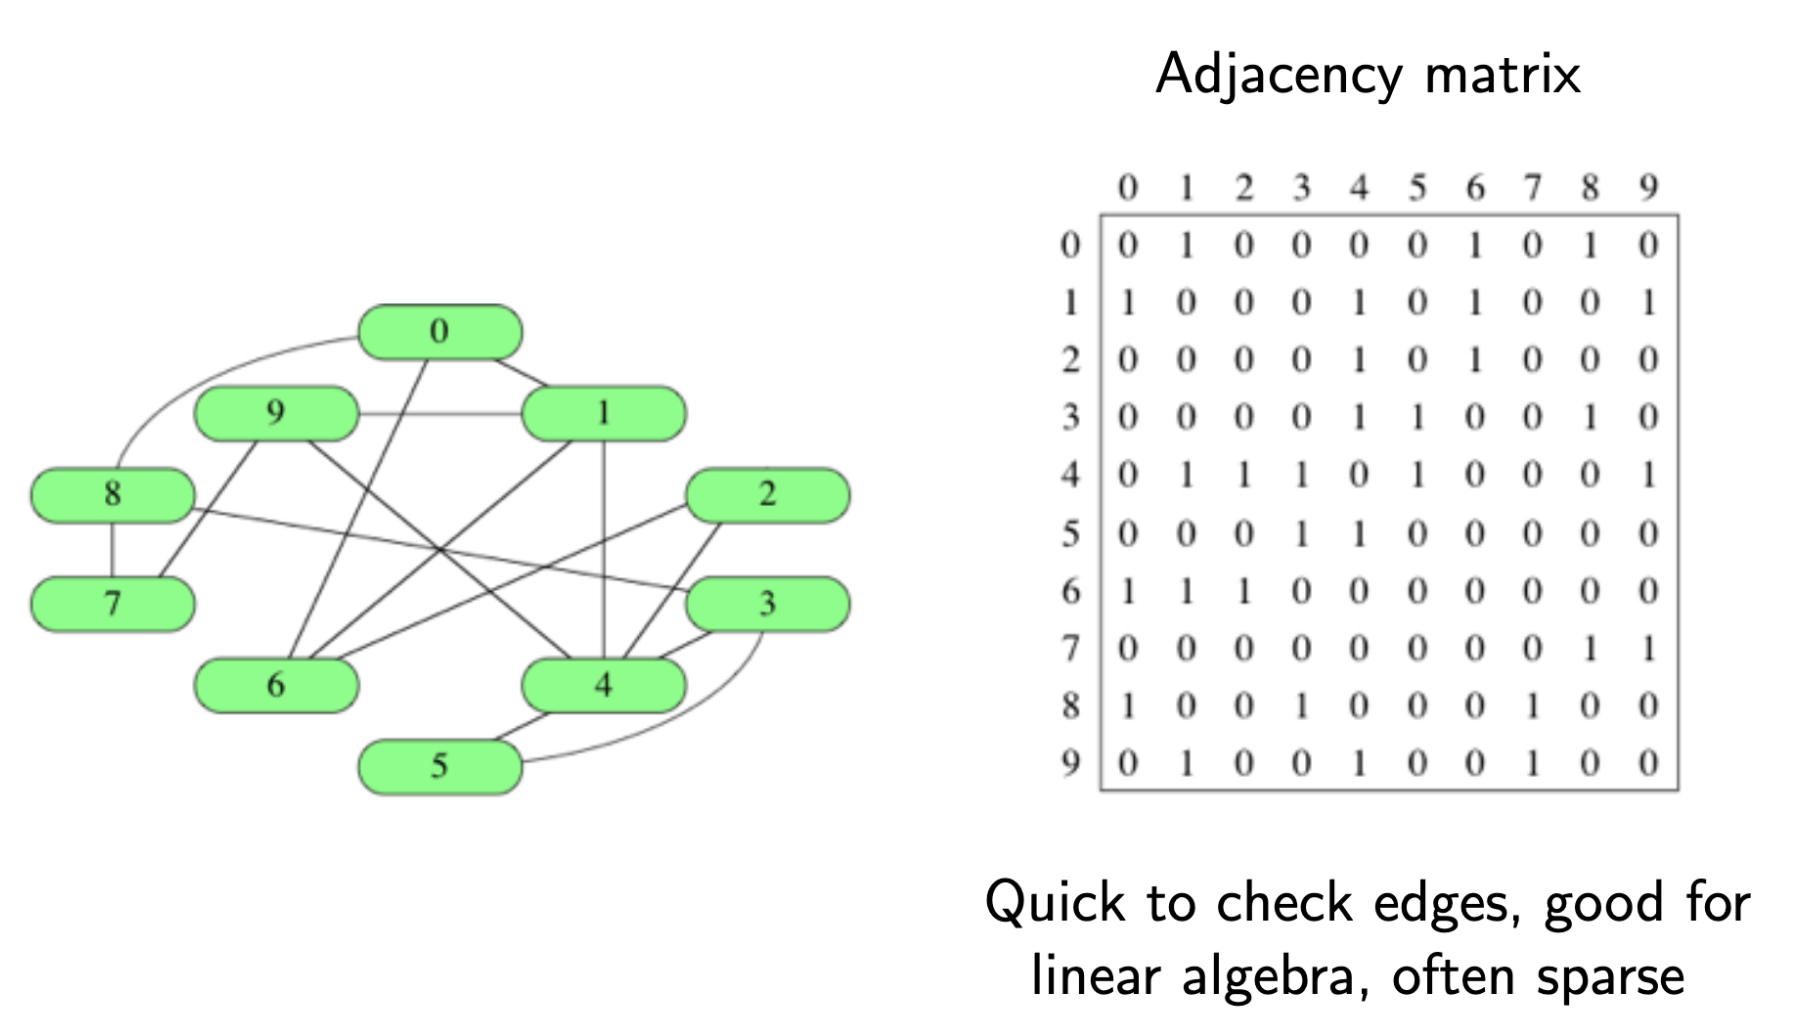
\includegraphics[width=0.5\textwidth]{figures/adjacency_matrix.png}
    \caption{
      A network with 10 vertices (left) and the adjacency matrix representation of its edges (right).}
    \label{fig:adjacency_matrix}
  \end{center}
\end{figure}

\subsection{Adjacency List}
The last data structure we covered, adjacency list is a combination of edge list and adjacency matrix. An adjacency list of a network with $|V|$ vertices has length $|V|$ where each element i is a list of vertices adjacent to vertex i. The space complexity of an adjacency matrix is $\Theta(E)$ where $|E|$ is the number of edges in the network. Checking whether a vertex i has an edge to vertex j takes $O(d)$ time where d is the degree of the vertex i.

\begin{figure}[ht]
  \begin{center}
    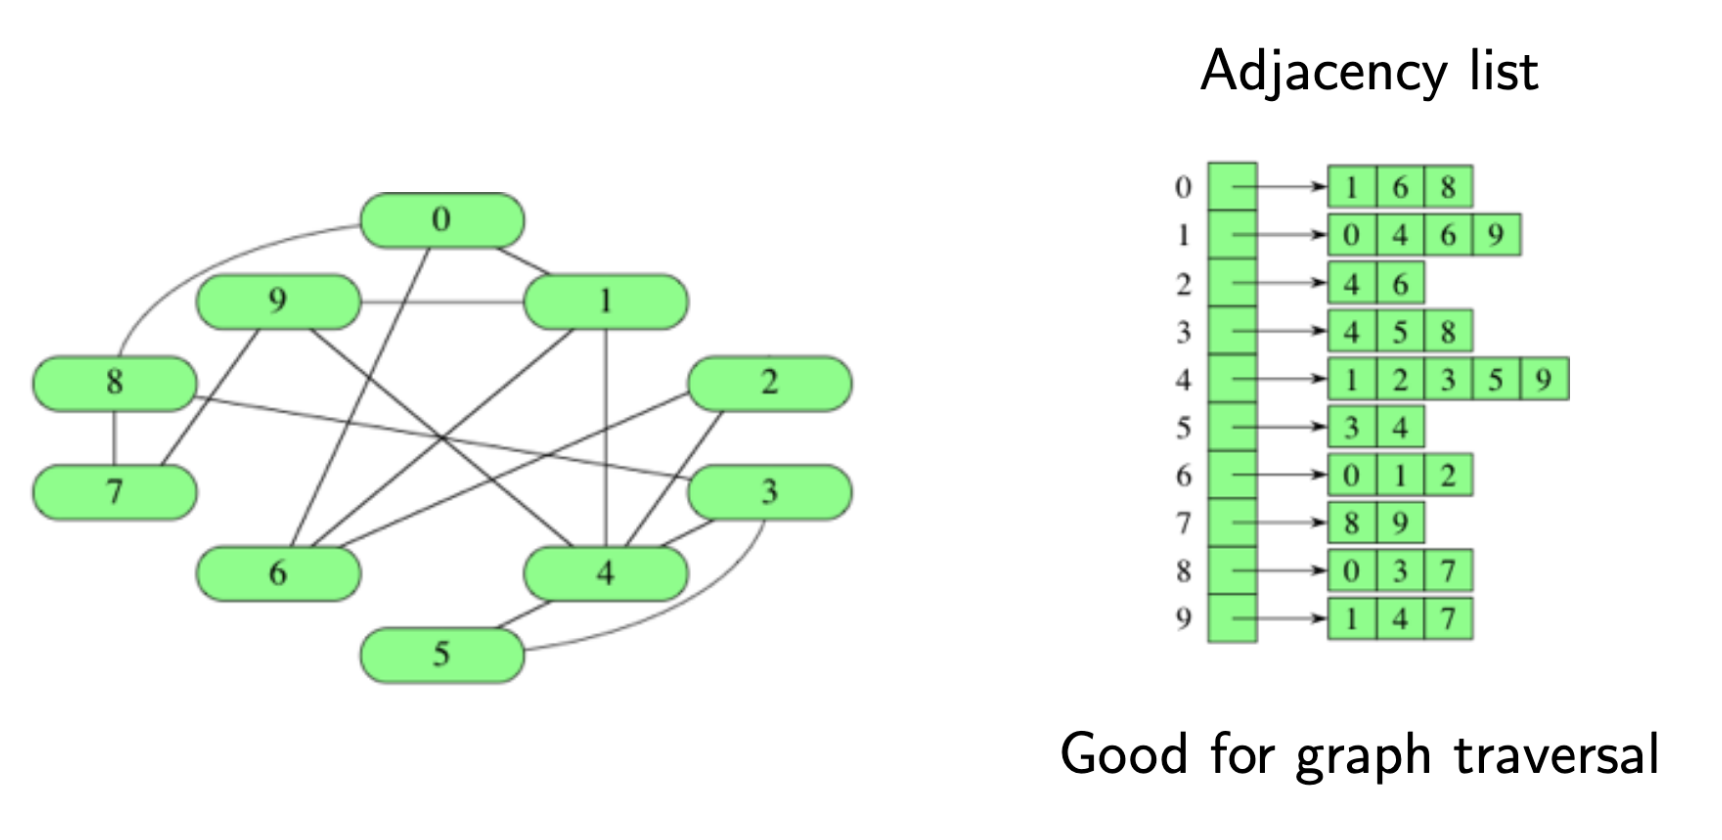
\includegraphics[width=0.5\textwidth]{figures/adjacency_list.png}
    \caption{
      A network with 10 vertices (left) and the adjacency list representation of its edges (right).}
    \label{fig:adjacency_list}
  \end{center}
\end{figure}

Note: See Networks.Rmd for the representation of some toy and real networks as various data structures using igraph.

\section{Network Topologies and Watts-Strogatz Networks}
While going over the capabilities of igraph, an R library (see Networks.Rmd), we learned about several network topologies (Figures \ref{fig:star}, \ref{fig:lattice} and \ref{fig:ring}) and generated some small world networks using a random graph generation model called the Watts-Strogatz model (Figures \ref{fig:small}, \ref{fig:medium}, and \ref{fig:large}).

\begin{figure}
\centering
\begin{minipage}{.3\textwidth}
  \centering
  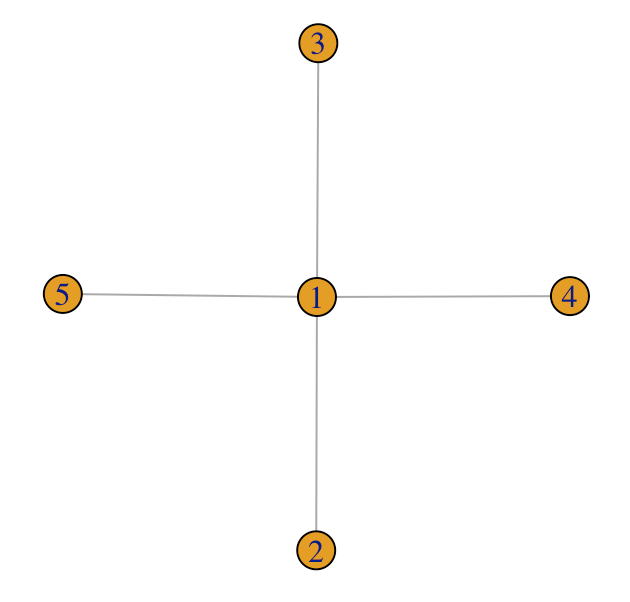
\includegraphics[width=.7\linewidth]{figures/star.png}
  \caption{Star Network}
  \label{fig:star}
\end{minipage}%
\begin{minipage}{.3\textwidth}
  \centering
  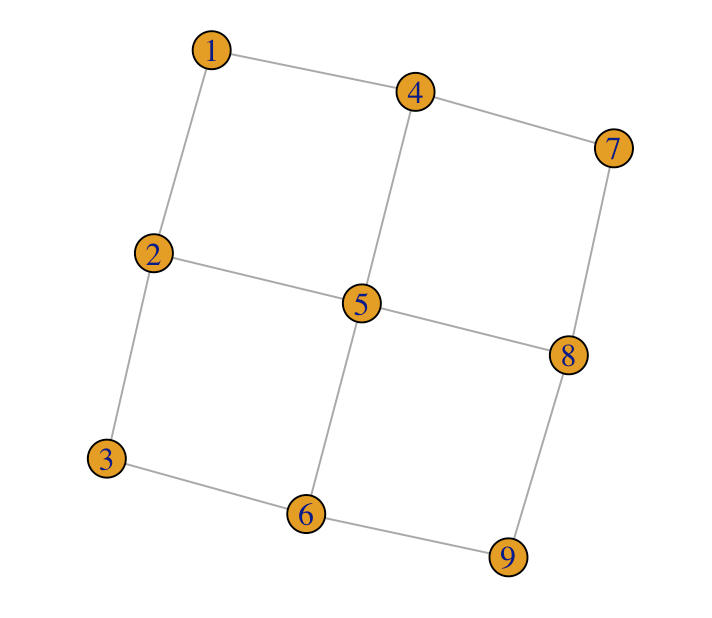
\includegraphics[width=.7\linewidth]{figures/lattice.png}
  \caption{Lattice Network}
  \label{fig:lattice}
\end{minipage}
\begin{minipage}{.3\textwidth}
  \centering
  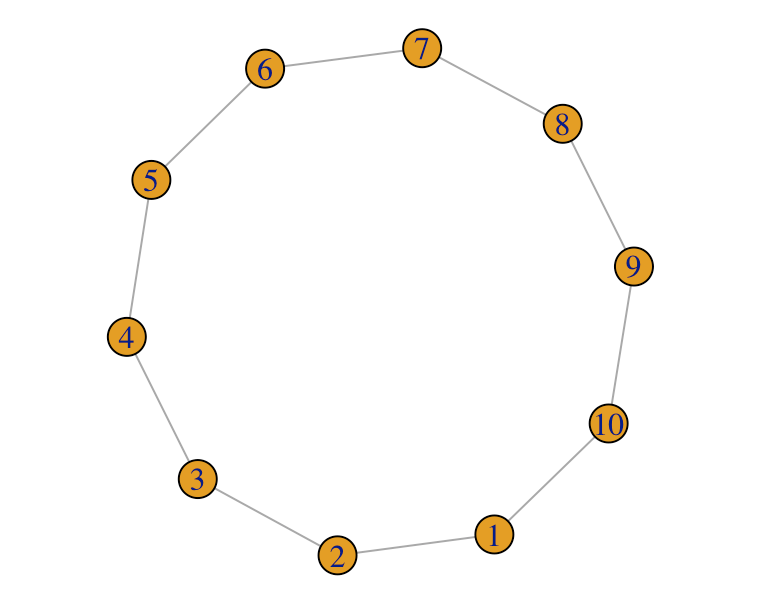
\includegraphics[width=.7\linewidth]{figures/ring.png}
  \caption{Ring Network}
  \label{fig:ring}
\end{minipage}
\end{figure}

\begin{figure}
\centering
\begin{minipage}{.3\textwidth}
  \centering
  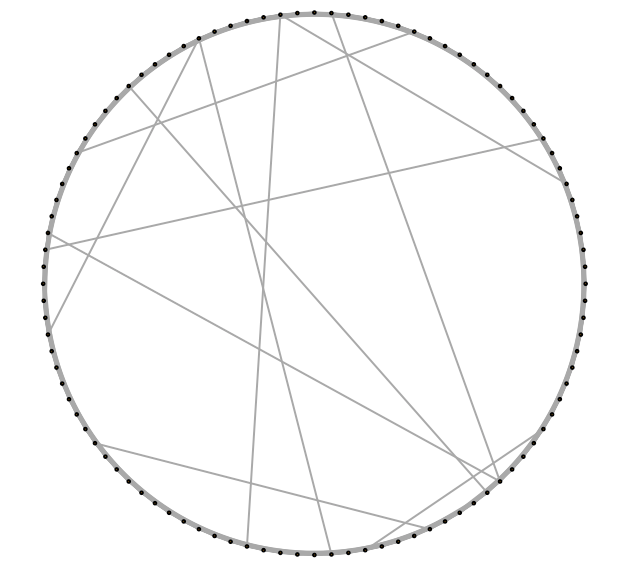
\includegraphics[width=.7\linewidth]{figures/small.png}
  \caption{Mostly a ring}
  \label{fig:small}
\end{minipage}%
\begin{minipage}{.3\textwidth}
  \centering
  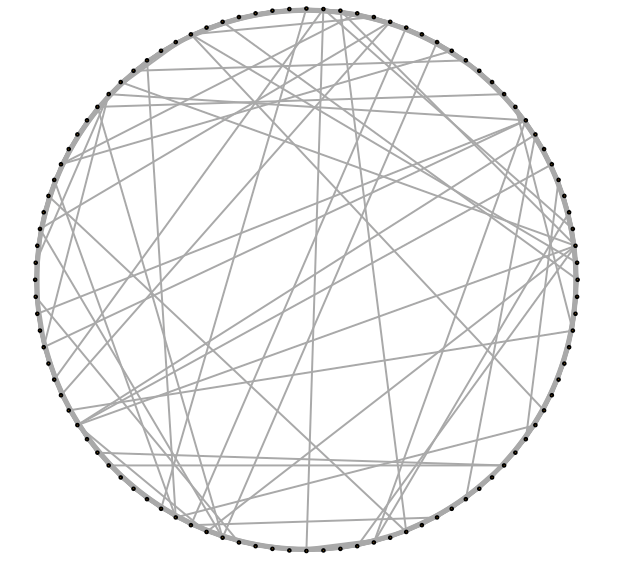
\includegraphics[width=.7\linewidth]{figures/medium.png}
  \caption{Some rewiring}
  \label{fig:medium}
\end{minipage}
\begin{minipage}{.3\textwidth}
  \centering
  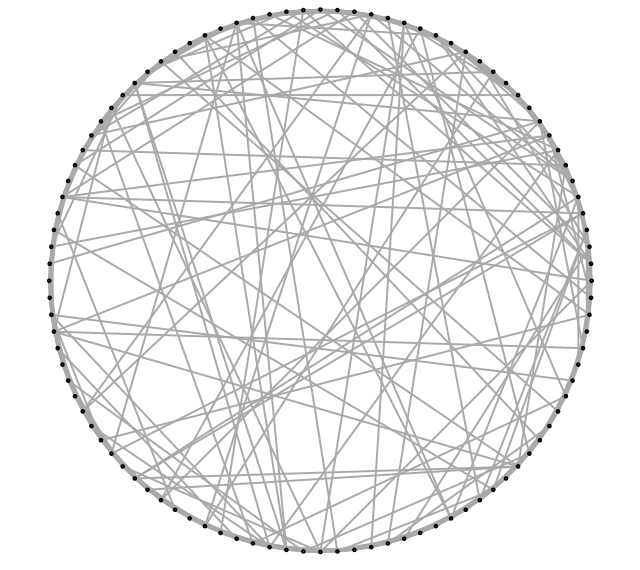
\includegraphics[width=.7\linewidth]{figures/large.png}
  \caption{Lots of rewiring}
  \label{fig:large}
\end{minipage}
\end{figure}

\section{Describing Networks}
Higher the dimension and complexity of a network, harder it gets to visualize. We discussed four different statistics for describing and analyzing a network, and algorithms one can use to calculate these statistics:
\begin{itemize}
  \item Degree: How many connections does a node have?
  \begin{itemize}
    \item Degree distributions
  \end{itemize}
  \item Path Length: What's the shortest path between two nodes?
  \begin{itemize}
    \item Breadth first search
  \end{itemize}
  \item Clustering: How many friends of friends are also friends?
  \begin{itemize}
    \item Triangle counting
  \end{itemize}
  \item Components: How many disconnected parts does the graph have?
  \begin{itemize}
    \item Connected components
  \end{itemize}
\end{itemize}

\subsection{Degree Distributions}
The degree of a node in a network is the number of connections it has to other nodes. The degree distribution of a network is the probability distribution of these degrees across the entire network. Working with some real life networks, we plotted some degree distributions and learned ways to make these plots more readable (See Networks.Rmd). Below are the code for and the visualization of the out-degree distribution (edges coming out of nodes) of the Wikipedia voting network and its log visualization: 

\begin{figure}[ht]
  \begin{center}
    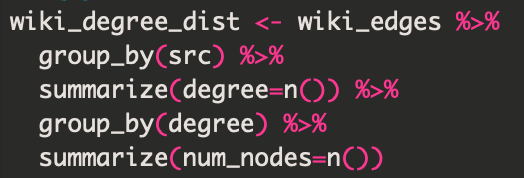
\includegraphics[width=0.5\textwidth]{figures/deg-dist.png}
    \caption{R code for out-degree distribution}
    \label{fig:deg-dist}
  \end{center}
\end{figure}

\begin{figure}
\centering
\begin{minipage}{.5\textwidth}
  \centering
  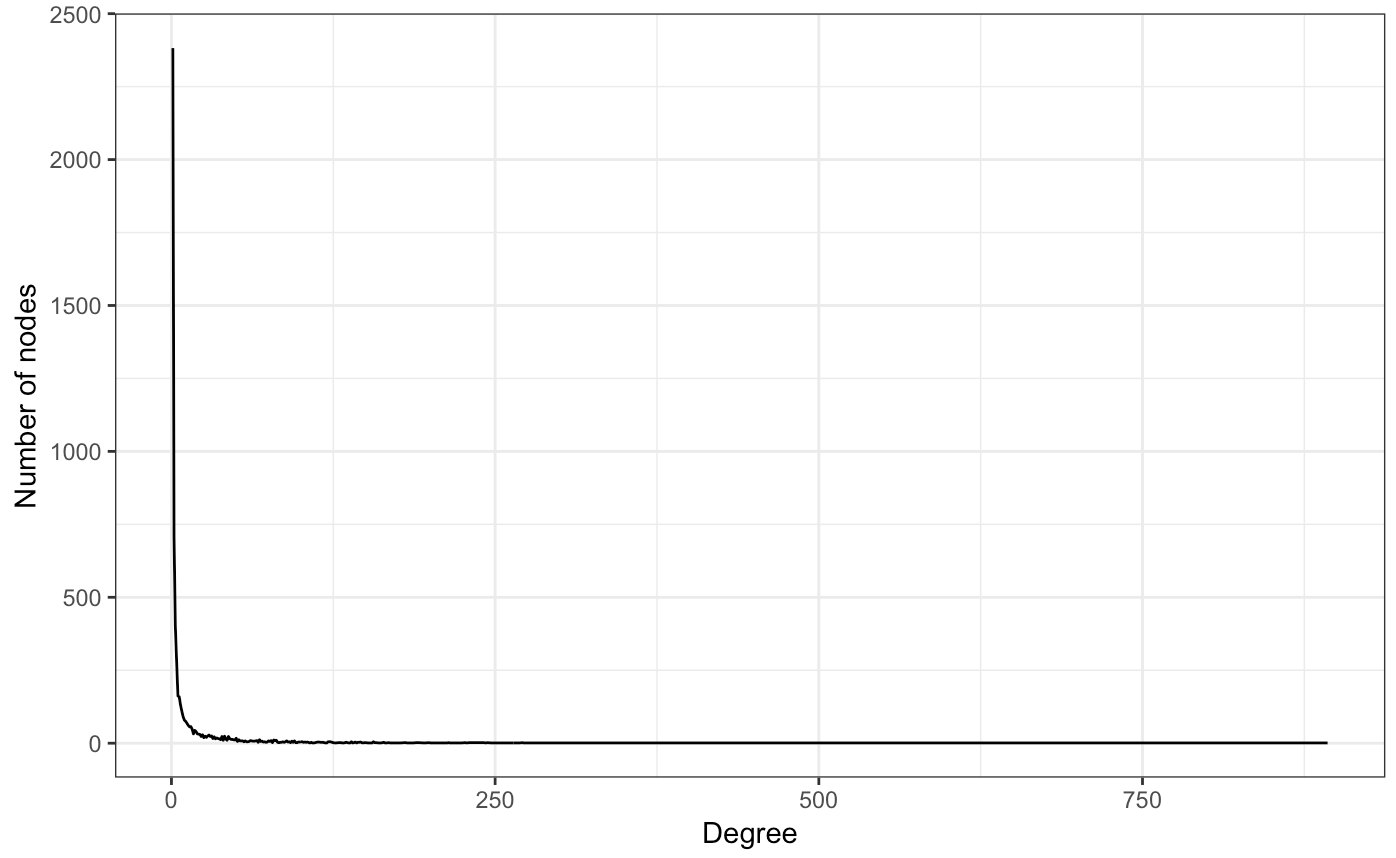
\includegraphics[width=.9\linewidth]{figures/out-deg.png}
  \caption{Visualization of Out-Degree Distribution}
  \label{fig:out-deg}
\end{minipage}%
\begin{minipage}{.5\textwidth}
  \centering
  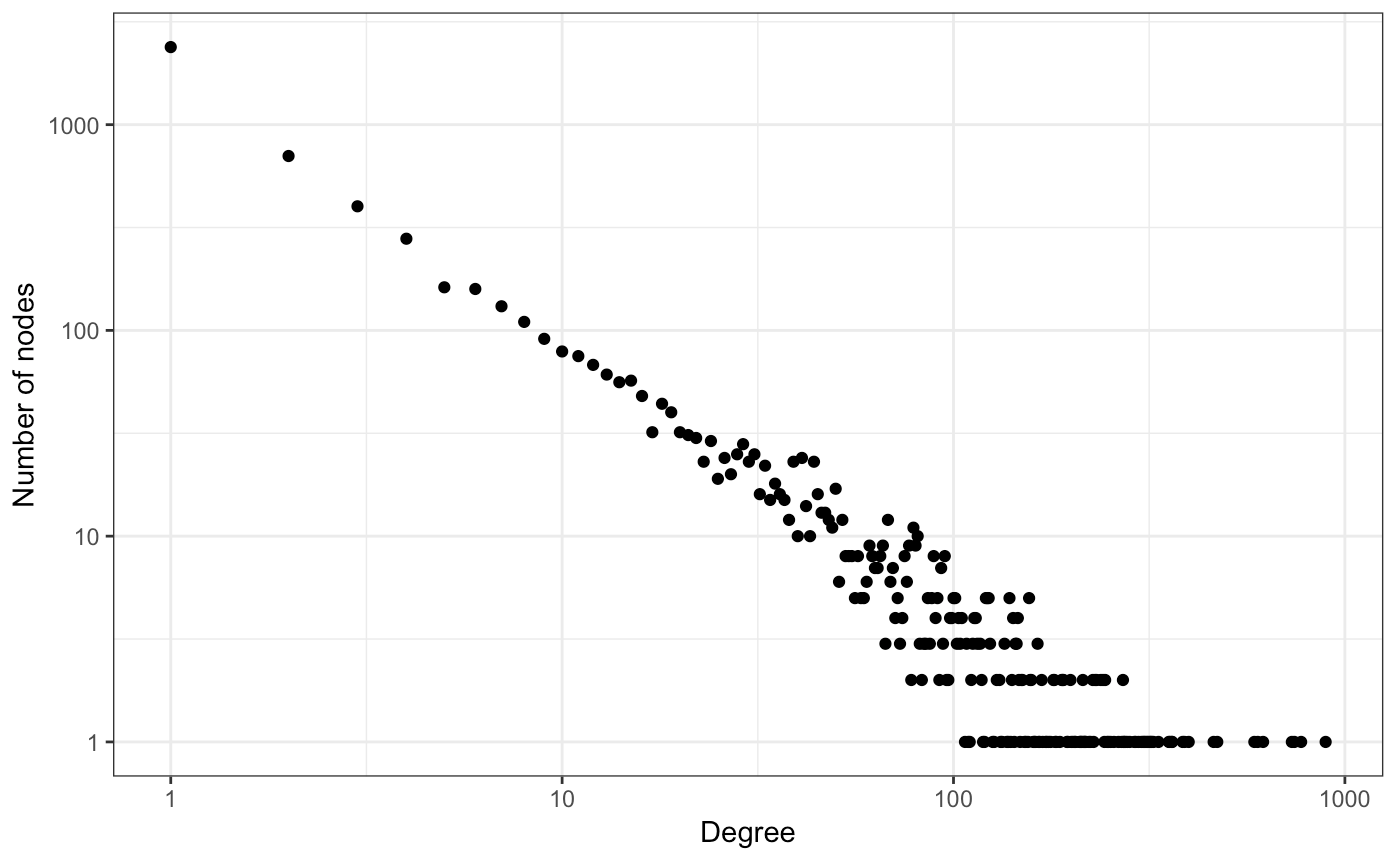
\includegraphics[width=.9\linewidth]{figures/out-deg-log.png}
  \caption{Visualization of Out-Degree Log Distribution}
  \label{fig:out-deg-log}
\end{minipage}
\end{figure}

\newpage
\subsection{Path Length}
Path length is the shortest distance between two nodes of a network. The path length distribution of a network is the distribution of the shortest paths between all node pairs in the network (See Network.Rmd for igraph way of calculating path lengths of a network and its visualization). The mean and median path lengths of a network are useful ways to analyze and understand a network. To calculate single-source shortest paths to all other nodes of a network, we can use an algorithm called Breadth First Search:
\subsubsection*{Breadth First Search}
Initialize all node distances to infinitely far \newline
Set source node distance to zero \newline
Initialize current boundary as source node \newline \newline
While current boundary is not empty: \{ \newline
Create empty list for new boundary \newline
For each node in current boundary: \{ \newline
loop over undiscovered neighbors and set neighbor distance as current distance+1 and add neighbor to the next boundary \newline
\} \newline
Set current boundary = next boundary \newline
\} \newline \newline
Note: See counting\_on\_networks.Rmd for BFS R code.
\subsection{Connected Components}
In a network, a connected component is a subgraph in which any two nodes are connected to each other by paths, and which is connected to no additional nodes in the overall graph. The algorithm to determine the connected components in a network uses BFS and is therefore fairly straightforward.

\begin{figure}[ht]
  \begin{center}
    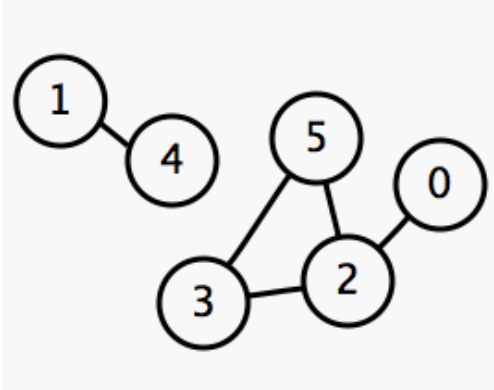
\includegraphics[width=0.3\textwidth]{figures/cc.png}
    \caption{
      A network with two connected components.}
    \label{fig:cc}
  \end{center}
\end{figure}

\subsubsection*{Connected Components Algorithm}
(1) Choose any node and perform BFS, labeling all the other nodes accessible from the chosen source node as component x. \newline
(2) Update label, choose any unlabeled node in the network and repeat (1) until all nodes are labeled.

\subsection{Clustering}
Clustering is the task of grouping a set of objects in such a way that objects in the same group are more similar to each other than to those in other groups. One way to think about it is in terms of mutual friends (connected nodes). How many friends of friends are also friends? For this end, we covered an algorithm referred to as triangle counting (See counting\_on\_networks.Rmd).

\subsubsection*{Counting Triangles}
Initialize counter for the number of triangles at each node \newline
Loop over each node: \{ \newline
Get the list of friends for node \newline
Add a count of 1 for each pair of node's friends that are connected \newline
\} \newline
\newpage
\section{Causality and (Natural) Experiments}
We started the new topic with a discussion on the difference between 'Prediction' and 'Causation'. We concluded that while 'Prediction' focuses on observing an environment and forecasting what is going to happen based on observation, 'Causation' focuses on changing the environment and anticipating the effects.

\begin{figure}[ht]
  \begin{center}
    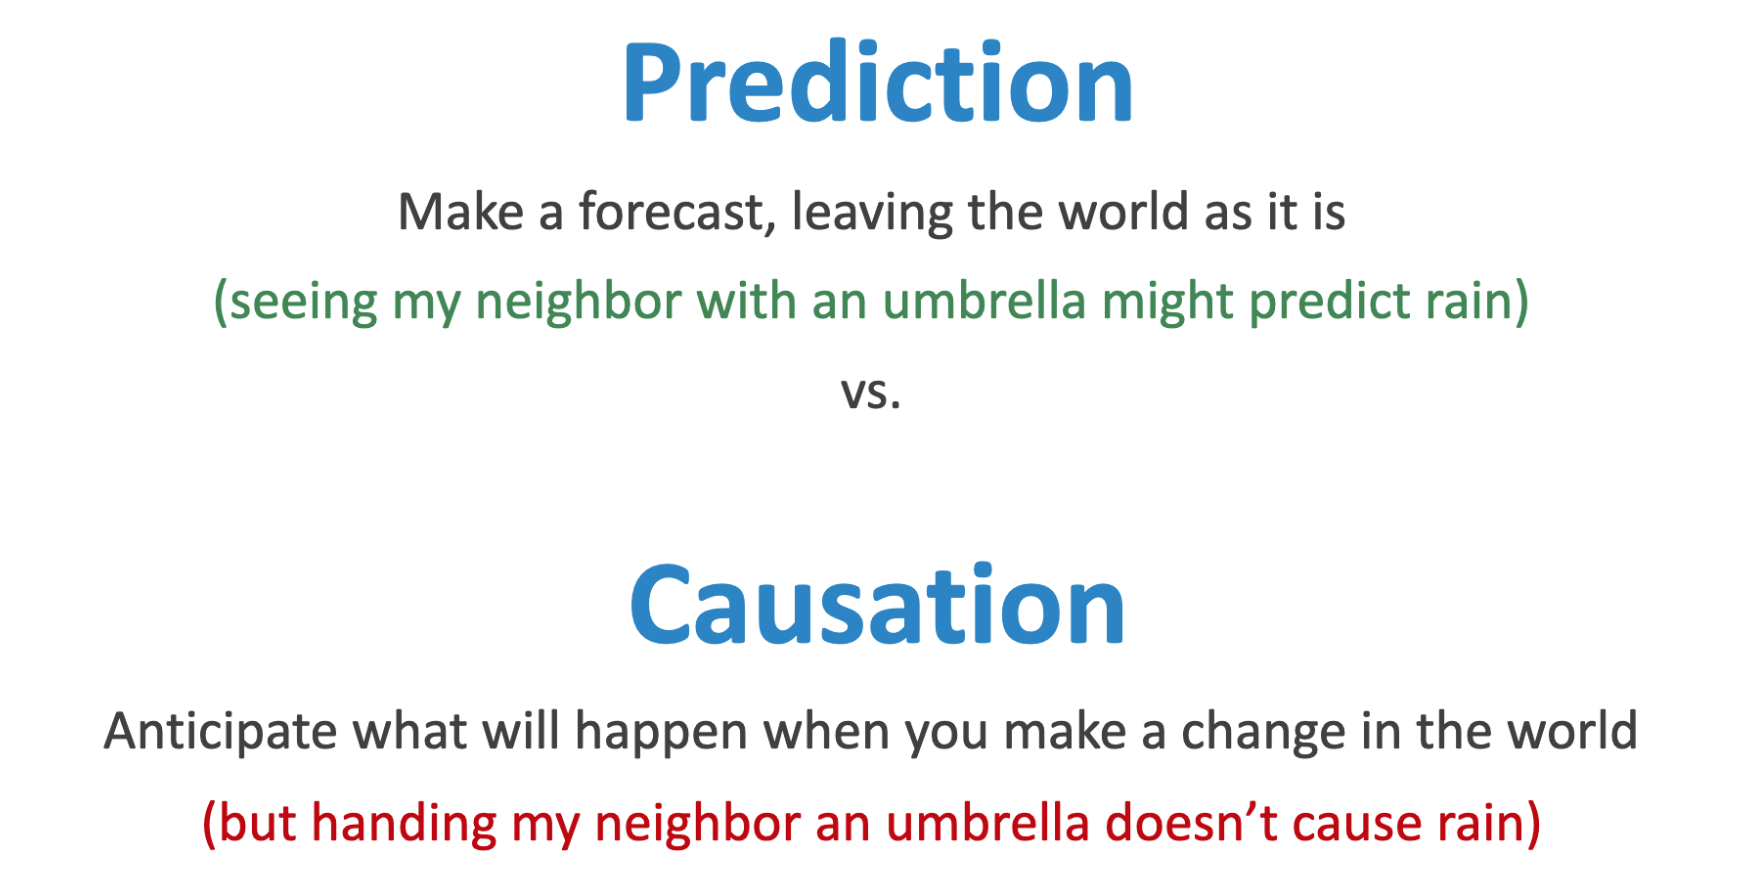
\includegraphics[width=0.5\textwidth]{figures/pred-caus.png}
    \caption{Prediction versus Causation}
    \label{fig:pred-caus}
  \end{center}
\end{figure}

Then we looked at the difference between 'Reverse Causal Inference' (causes of effects) and 'Forward Causal Inference' (effects of causes). While 'Reverse Causal Inference' is questioning 'What caused Y?', 'Forward Causal Inference' is asking 'What are the effects of X?'. In general, 'Forward Causal Inference' is easier than 'Reverse Causal Inference'. \newline \newline
Examples of 'Reverse Causal Inference':
\begin{itemize}
  \item What makes an email spam?
  \item What caused my kid to get sick?
  \item Why did the stock market drop?
\end{itemize}
Examples of 'Forward Causal Inference':
\begin{itemize}
  \item How does education impact future earnings?
  \item What is the effect of advertising on sales?
  \item How does hospitalization effect health?
\end{itemize}

We then took a closer look at the last example, 'How does hospitalization effect health?':

\begin{figure}[ht]
  \begin{center}
    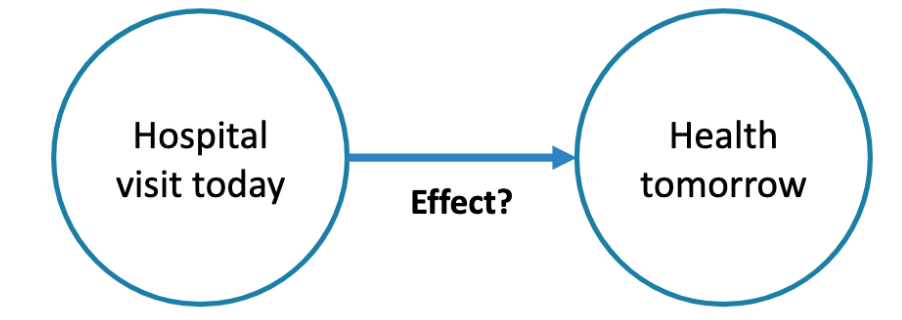
\includegraphics[width=0.5\textwidth]{figures/hos-health.png}
    \caption{Arrow means 'X causes Y'}
    \label{fig:hos-health}
  \end{center}
\end{figure}

As we discussed in class, this representation of the cause-effect relationship between going to the hospital today and one's health tomorrow can lead to a problematic conclusion: Going to the hospital makes you sick. In such a case, regardless of how many observations one might have, the conclusions one draws will be biased. Thus, this relationship cannot be explained independently of some other common factor.

\subsubsection*{Confounds}
The effect and cause might be confounded by a common cause and be changing together as a result. In fact, there could be many confounds. Going back to our hospital/health example, it is easy to recognize that visiting the hospital today and one's health tomorrow both depend on another cause, one's health today. If one only observes the cause and effect changing together, one cannot estimate the effect of hospitalization alone on health tomorrow.

\begin{figure}[ht]
  \begin{center}
    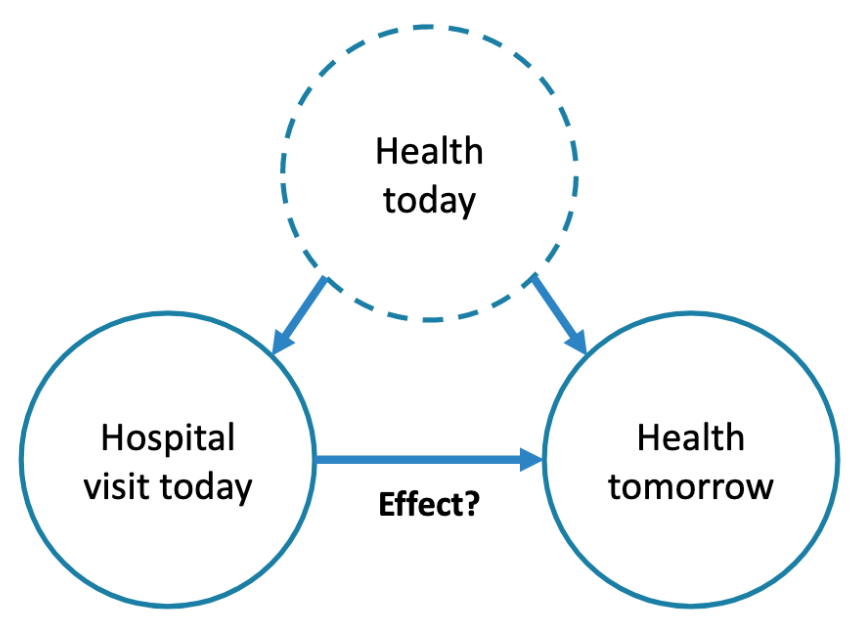
\includegraphics[width=0.5\textwidth]{figures/confounds.png}
    \caption{Dashed circle means 'unobserved'.}
    \label{fig:confounds}
  \end{center}
\end{figure}

\subsubsection*{Observational Estimates}
Let us say all sick people in our dataset went to the hospital today and healthy people stayed at home. The observed difference in health tomorrow is:

\begin{figure}[ht]
  \begin{center}
    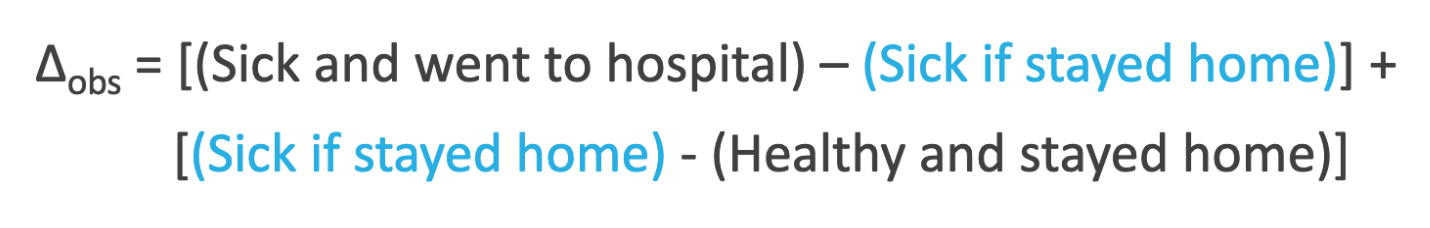
\includegraphics[width=0.5\textwidth]{figures/obs-diff.png}
    \caption{Here we are trying to compare something that did happen with something that could have happened. Unfortunately, we cannot clone people and make their clones stay at home.}
    \label{fig:obs-diff}
  \end{center}
\end{figure}

\subsubsection*{Selection Bias}
Selection bias is the baseline difference between those who opted in to the treatment and those who did not.

\begin{figure}[ht]
  \begin{center}
    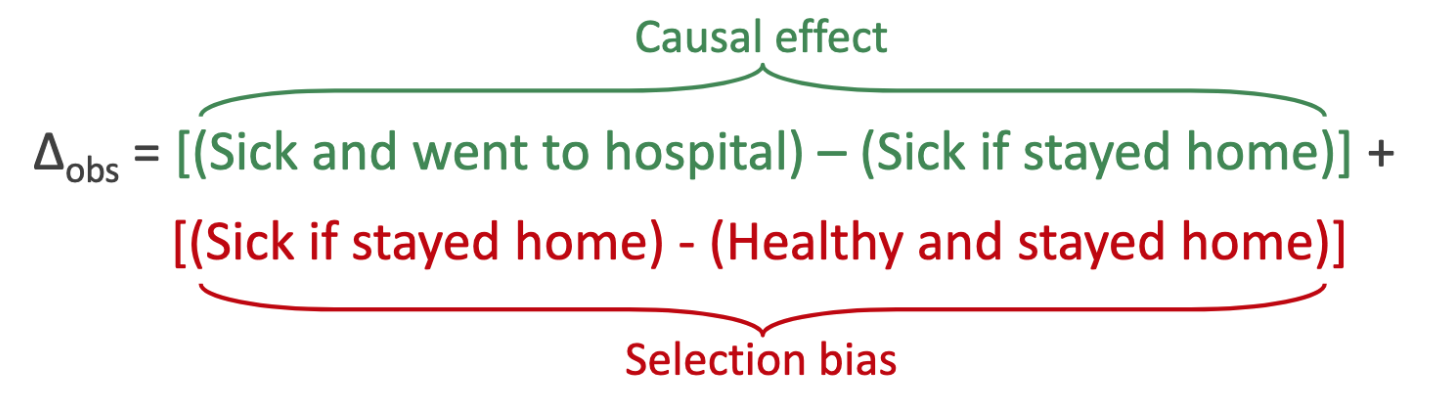
\includegraphics[width=0.5\textwidth]{figures/sel-bias.png}
    \caption{Selection bias is likely negative here, making the observed difference an underestimate of the causal effect.}
    \label{fig:sel-bias}
  \end{center}
\end{figure}

\subsubsection*{Simpson's Paradox}
Selection bias can be so large that observational and causal estimates give opposite effects (e.g. going to the hospital makes you sick). This is called the Simpson's Paradox.

\begin{figure}[ht]
  \begin{center}
    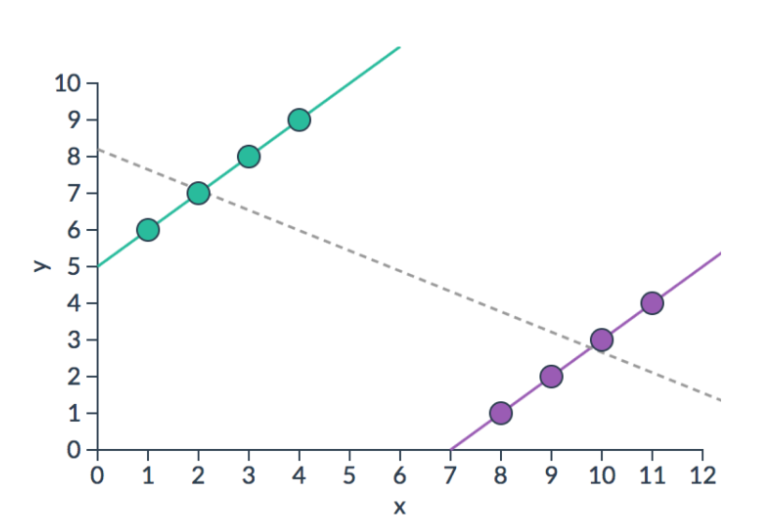
\includegraphics[width=0.5\textwidth]{figures/simp.png}
    \caption{Simpson's Paradox}
    \label{fig:simp}
  \end{center}
\end{figure}

\subsection*{Controlled Experiments}
\subsubsection*{Counterfactuals}
To isolate the causal effect, we have to change one and only one thing (hospital visits) and compare the outcomes. Unfortunately, we never get to observe what would have happened if we did something else so we have to estimate it.

\begin{figure}[ht]
  \begin{center}
    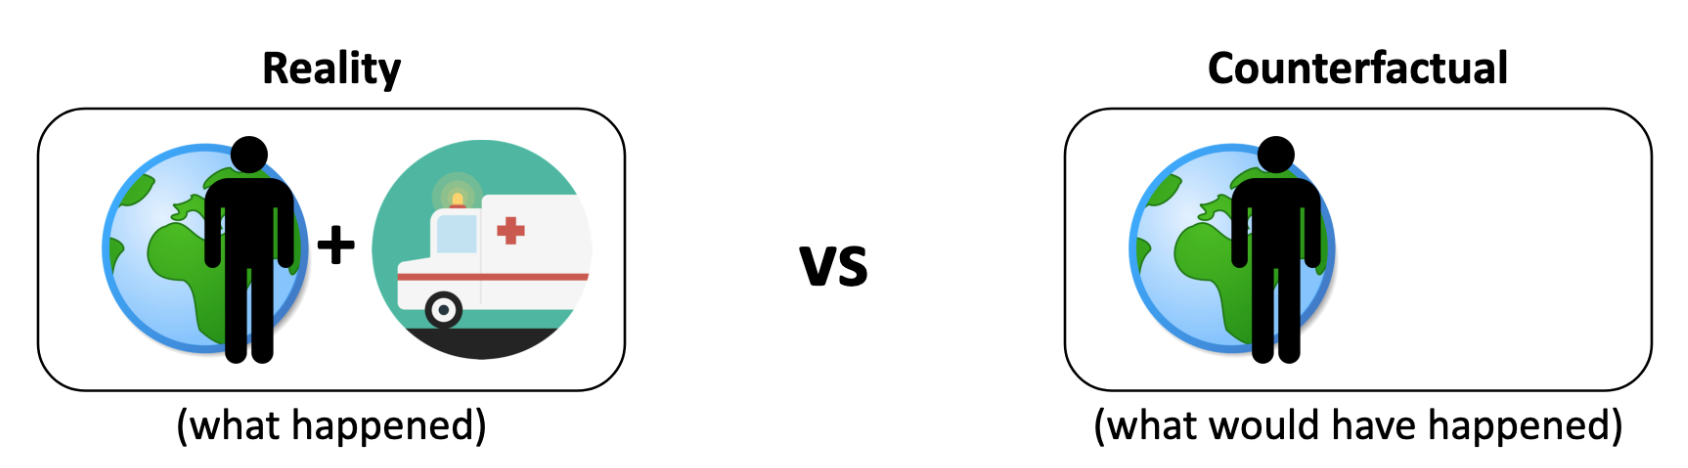
\includegraphics[width=0.5\textwidth]{figures/counter.png}
    \caption{Reality versus Counterfactual}
    \label{fig:counter}
  \end{center}
\end{figure}

\newpage
\subsubsection*{Random Assignment}
We cannot clone people but by randomly assigning their actions with a coin flip, we can get results almost as good as cloning. In the hospital example, we can use randomization to create two groups that differ only in which treatment they receive. This allows us to restore symmetry.

\begin{figure}[ht]
\centering
    \begin{subfigure}
        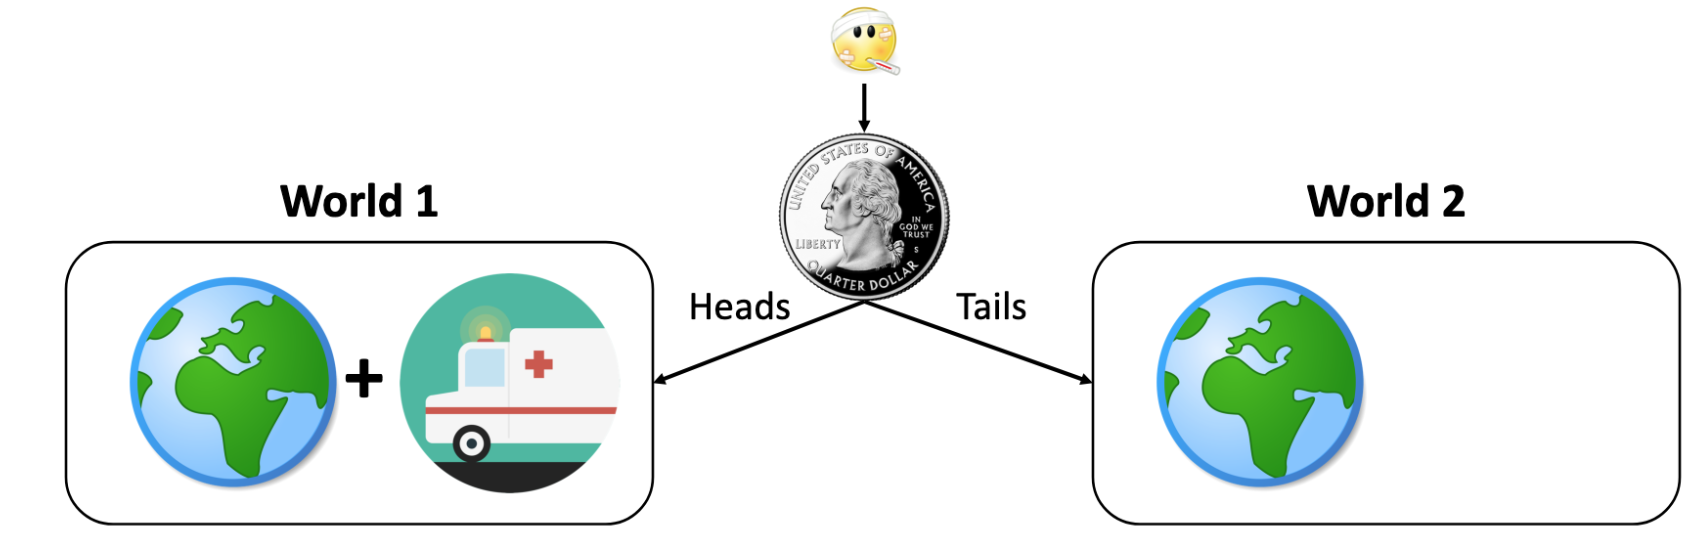
\includegraphics[width=0.5\textwidth]{figures/random.png}
        \caption{Randomly assign both sick and healthy people to which treatment they will receive.}
        \label{fig:random}
    \end{subfigure}
    \begin{subfigure}
        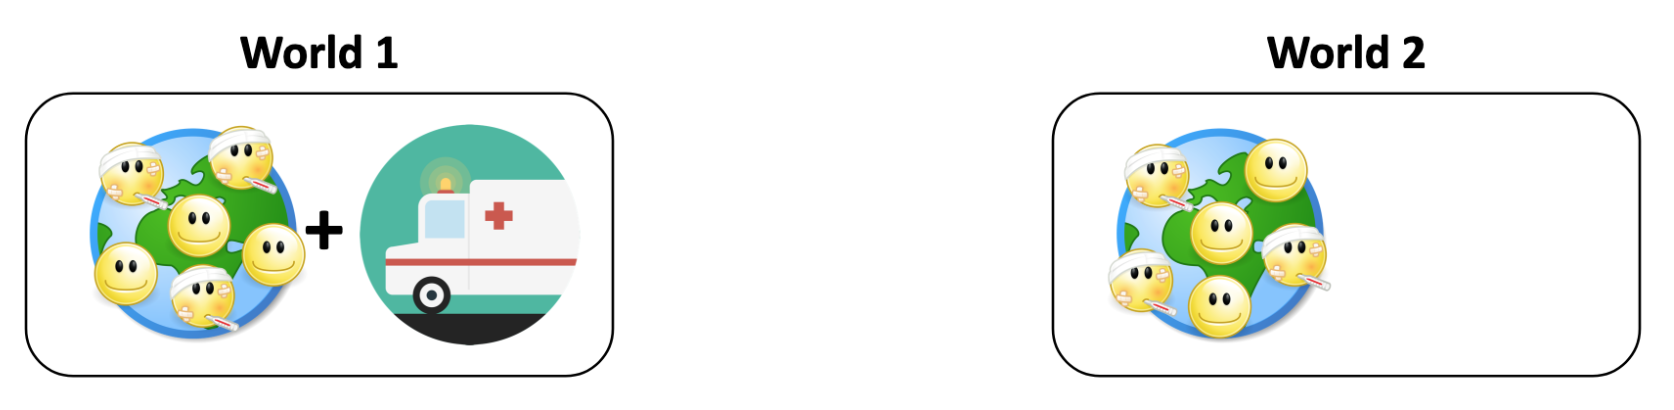
\includegraphics[width=0.5\textwidth]{figures/worlds.png}
        \caption{The resulting worlds closely resemble the reality versus counterfactual separation we desire.}
        \label{fig:worlds}
    \end{subfigure}
\end{figure}

\end{document}

%%% Local Variables:
%%% mode: latex
%%% TeX-master: t
%%% End:
